% An echo-type sequence applied to the root pulse partially mitigates decoherence effects but remains limited by pronounced amplitude-dependent broadening. Conversely, the Lorentzian echo variant demonstrates an amplitude-independent linewidth spanning over three orders of magnitude in drive strength, evidencing remarkable robustness against amplitude-induced dephasing. This insensitivity arises from the adiabatic evolution and the symmetric frequency-splitting intrinsic to the pulse design. The primary limitation lies in the floating offset and amplitude-dependent baseline, resulting in reduced contrast compared to conventional square and Lorentzian drives.



To identify the useful operating regime, we examine the linewidth and contrast
of the echo response as functions of pulse duration and drive amplitude.  We
choose pulse durations shorter than $T_1$, but long enough that Fourier
broadening does not dominate.  The duration-dependent linewidth, contrast,
and contrast-weighted resolution are reported in the Supplemental
Material~\cite{SupplementalMaterial}.

A second design constraint is the cutoff of the formally infinite-support
pulse envelope.  Truncation introduces a residual endpoint drive
$\Omega_c=c\Omega_0$ and a corresponding cutoff-broadening
contribution~\cite{boradjiev_qubit_2013,mihov_defying_2024,mihov_qubit_2024}.
The relevant weak-saturation condition is
$s_c=\Omega_c^2T_1T_2\ll1$, or
$\Omega_c\ll1/\sqrt{T_1T_2}$; the inequality therefore points toward
\emph{smaller}, not larger, endpoint amplitudes.  The relative cutoff $c$
cannot be specified independently of $\Omega_0$, $T_1$, and $T_2$, giving a
three-dimensional design space of pulse duration, drive amplitude, and cutoff
level.

The waveform itself offers a further control of the linewidth--contrast
tradeoff. A derivative removal by adiabatic gate (DRAG) pulse adds a
quadrature component proportional to the time derivative of the in-phase
waveform to suppress leakage and drive-induced phase
errors~\cite{motzoi_drag_2009,gambetta_analytic_2011}.
Figure~\ref{fig:pulse-improvement} compares three-level simulations
for a $30~\mu\mathrm{s}$ echo-root-Lorentzian pulse with $c=0.001$: an uncorrected outer
envelope, the same envelope with DRAG, and DRAG with a polynomial edge
correction. All three use the same sine-smoothed phase jump $s(t)$ of
duration $T_s=16~\mathrm{ns}$ at the midpoint. The corrected pulse is
\begin{align}
    L_{\mathrm{floor}}^{(1/2)}(t)
    &=\frac{L^{(1/2)}(t)-c}{1-c},\\
    W_p(t)&=\left[1-\left(\frac{2t}{L}\right)^2\right]^p,
    \qquad p=5,\\
    s(t)&=\begin{cases}
        +1, & t\leq-T_s/2,\\
        -\sin(\pi t/T_s), & |t|<T_s/2,\\
        -1, & t\geq T_s/2,
    \end{cases}\\
    L^{\mathrm{smooth}}(t)
    &=L_{\mathrm{floor}}^{(1/2)}(t)\,s(t)\,W_p(t).
\end{align}
Here $|t|<L/2$, $\tau=(L/2)/\sqrt{c^{-2}-1}$, and $W_p=0$ outside
the pulse. The floor correction removes the endpoint offset, and
$W_p(t)$ smooths the edges. Thus, (a)--(b) isolate DRAG,
while (b)--(c) isolate this edge correction.
With $I(t)=\Omega_0L^{\mathrm{smooth}}(t)$, the added DRAG
quadrature is
\begin{equation}
    Q(t)=-\frac{\beta}{|\alpha|}\frac{dI(t)}{dt},
    \label{eq:drag-quadrature}
\end{equation}
where $\alpha=\omega_{12}-\omega_{01}$ is the qubit anharmonicity.
We use DRAG with $\beta=-0.5$ for near-optimal compensation of
AC-Stark-induced detuning~\cite{motzoi_drag_2009,gambetta_analytic_2011},
as supported by the coefficient scan in the Supplemental
Material~\cite{SupplementalMaterial}.

DRAG suppresses amplitude-dependent resonance motion: the interpolated
center RMS falls from $6.54~\mathrm{kHz}$ for the echo to
$0.31~\mathrm{kHz}$ with DRAG and $0.29~\mathrm{kHz}$ with DRAG plus
the polynomial correction [Fig.~\ref{fig:pulse-improvement}(d)].
These sub-grid estimates quantify the saved maps; they do not independently
establish sub-kHz numerical accuracy.
DRAG does not, by
itself, prevent the high-drive linewidth increase in this comparison.
Adding the polynomial correction changes the FWHM at
$\Omega_0/(2\pi)=100~\mathrm{MHz}$ from $506$ to $162~\mathrm{kHz}$,
while the probability contrast increases from $0.079$ to $0.315$.
The corrected pulse maintains contrast above $0.31$ across the sampled
$10$--$100~\mathrm{MHz}$ range. This improvement comes at the cost of a
broader low-drive line, and the high-drive width remains above
$1/(\pi T_2)$. Here contrast is the dip depth relative to the local
background, expressed as a probability difference rather than normalized
by measurement noise.
These simulations establish a pulse-shaping tradeoff rather than an
experimental sensitivity gain or a globally optimized waveform.

Figure~\ref{fig:duration-cutoff-scan} maps the joint dependence on cutoff
and drive amplitude for the $30~\mu\mathrm{s}$ polynomial-corrected DRAG
echo. The white contours mark $C=0.2$: the band between them has a dip
depth exceeding 0.2 in excitation probability. Across this broad region
of parameter space, the simulated response combines appreciable contrast
with local FWHM values of $112$--$182~\mathrm{kHz}$, approximately
$2.6$--$4.2$ times the coherence reference $\Gamma_{T_2}$.
The contours select contrast; the linewidth within that region is read
independently from panel (a).

The useful band shifts toward smaller cutoff as drive increases, yet a
single cutoff can retain both narrow linewidth and high contrast over a
wide drive range. For example, at the sampled
$c=6.58\times10^{-4}$, the local FWHM remains below $155~\mathrm{kHz}$
and contrast above $0.32$ throughout the sampled $10$--$100~\mathrm{MHz}$
interval. Here $c$ sets the original root-Lorentzian core width even though
the corrected envelope vanishes at its endpoints: changing $c$ also
changes $\tau$. The full duration survey and numerical checks are given
in the Supplemental Material~\cite{SupplementalMaterial}.

% Let the text flow around Figure 4 without a forced page break.
\begin{figure}[t]
    \centering
    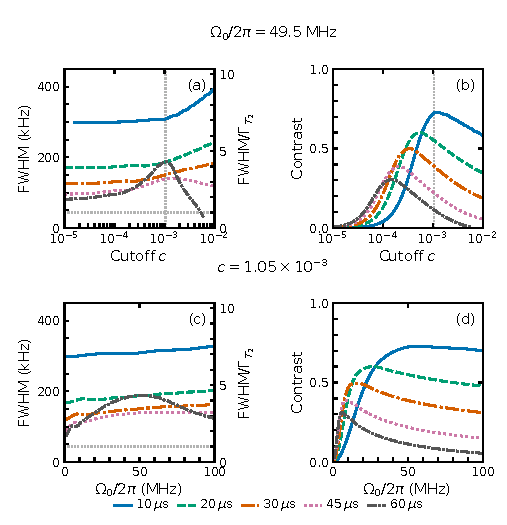
\includegraphics[width=\columnwidth]{../figures/paper/04_duration_cutoff_scan.pdf}
    \caption{Simulated cutoff and duration dependence of the polynomial-corrected DRAG echo.
    (a),(b) Normalized dip FWHM and contrast $C$ versus cutoff and drive
    amplitude for $L=30~\mu\mathrm{s}$.
    The white contours enclose the $C>0.2$ band, where panel (a) also
    shows narrow dips. Cutoff controls the pulse-core width; this band
    balances spectral narrowing against loss of contrast, retaining a
    distinguishable resonance over a broad amplitude range.
    (c),(d) Cutoff slices at $\Omega_0/(2\pi)=49.5~\mathrm{MHz}$
    (orange dashed lines) for durations $L=10$--$60~\mu\mathrm{s}$.
    The thick orange $30~\mu\mathrm{s}$ curves match the maps;
    dotted lines mark $\mathrm{FWHM}/\Gamma_{T_2}=1$ in (c) and $C=0.2$ in (d).}
    \label{fig:duration-cutoff-scan}
\end{figure}

